%% Paper for International Journal on Smart Grid
%% Reformatted from: Beyond Imbalance Ratio: Data Characteristics as Critical Moderators

\documentclass{ijSmartGrid}

%% ---- Additional packages (add as needed) ----
\usepackage{booktabs}      % Professional tables
\usepackage{array}         % Enhanced table column types
\usepackage{multirow}      % Multi-row table cells
\usepackage{algorithm}
\usepackage{algorithmic}
\usepackage{xcolor}
\usepackage{subcaption}    % Sub-figures
\usepackage{tikz}
\usetikzlibrary{positioning,arrows.meta}
\usepackage{amsthm}
\theoremstyle{definition}
\newtheorem{hypothesis}{Hypothesis}
\usepackage{hyperref}      % Clickable links in PDF (load last)
\hypersetup{
  colorlinks = true,
  linkcolor  = black,
  citecolor  = black,
  urlcolor   = black
}

%% ---- Custom hyphenation to prevent overflow ----
\hyphenation{over-sam-pling im-bal-anced sep-a-ra-bil-ity}

%% ============================================================
%%  TITLE BLOCK INFORMATION
%% ============================================================

\title{Beyond Imbalance Ratio: Data Characteristics as Critical Moderators of Oversampling Method Selection}

\author{%
  Jiangyuwen\textsuperscript{*}\orcidlink{0009-0001-4022-1436},
  Ye~Songyun\textsuperscript{**}\orcidlink{0009-0009-5048-3147}%
}

\ijaffiliation{%
  \textsuperscript{*}School of Artificial Intelligence,
    Guangzhou Institute of Science and Technology,
    Guangzhou, China \\
  \textsuperscript{**}School of Artificial Intelligence,
    Guangzhou Institute of Science and Technology,
    Guangzhou, China%
}

\ijemail{%
  jiangyuwen@gzist.edu.cn,
  yesongyun@gzist.edu.cn%
}

\corresponding{%
  \textsuperscript{\dag} Corresponding Author:
  Ye~Songyun,
  School of Artificial Intelligence,
  Guangzhou Institute of Science and Technology,
  Guangzhou, China,
  yesongyun@gzist.edu.cn%
}

\receivedaccepted{xx.xx.xxxx}{xx.xx.xxxx}

%% ============================================================
%%  RUNNING HEADER METADATA
%% ============================================================

\ijshortauthor{Jiangyuwen and Ye~Songyun}

\ijvolume{x}
\ijissue{x}
\ijpubmonth{Month}
\ijpubyear{xxxx}

\ijarticletype{Research Article}

%% ============================================================
%%  DOCUMENT BODY
%% ============================================================
\begin{document}

\maketitle

% Ensure paragraph indentation for all sections
\setlength{\parindent}{0.63cm}
\setlength{\parskip}{6pt}

%% ---- Abstract (max 250 words, no citations) ----
\begin{abstract}
\textbf{Background:} The IR-threshold paradigm assumes a positive correlation between imbalance ratio (IR) and oversampling effectiveness for method selection, yet this assumption lacks rigorous causal validation. \textbf{Methods:} We conducted 12 controlled experiments ($N>100$ dataset variants) manipulating IR while controlling data characteristics (separability, cluster structure) through algorithmic generation of Gaussian mixture datasets, supplemented by validation on 18 real-world datasets from OpenML. \textbf{Results:} Contrary to prevailing assumptions, IR exhibits a statistically significant negative correlation ($r=-0.68$, $p<0.001$, 95\% CI: $[-0.823, -0.451]$) with oversampling benefits when confounds are controlled. Class separability emerges as the strongest moderator ($\rho=-0.72$, $p=0.003$, 95\% CI: $[-0.891, -0.412]$), substantially outweighing IR's influence. \textbf{Conclusion:} Data characteristics, not IR alone, should guide oversampling method selection. Our ``Context Matters'' framework provides evidence-based selection criteria integrating IR, class separability, and cluster structure.
\end{abstract}

% Restore paragraph indentation after abstract
\setlength{\parindent}{0.63cm}
\setlength{\parskip}{6pt}

%% ---- Keywords (minimum 3, maximum 5) ----
\keywords{class imbalance, oversampling method selection, imbalance ratio, data characteristics, class separability}

%% ============================================================
%%  SECTION 1: INTRODUCTION
%% ============================================================
\section{Introduction}
\indent Class imbalance constitutes a fundamental challenge in machine learning applications spanning fraud detection, medical diagnosis, and cybersecurity. In these critical domains, minority class instances---typically the primary objects of interest---often represent less than 1\% of available data. This distributional skew induces substantial bias in standard classification algorithms, which optimize for aggregate accuracy and consequently favor majority class prediction, thereby impairing detection of rare but significant events.

To address this fundamental challenge, researchers have developed numerous methodological approaches, broadly categorized into three paradigms: data-level interventions (oversampling and undersampling), algorithm-level modifications (cost-sensitive learning and threshold optimization), and ensemble strategies \cite{chawla2002smote,he2008adasyn,ling1998decision,galar2012review}. Early investigations into the relative effectiveness of under-sampling versus over-sampling \cite{drummond2003c4,estabrooks2004multiple} highlighted the importance of experimental design in evaluating these approaches. Among these, synthetic oversampling---particularly the Synthetic Minority Over-sampling Technique (SMOTE) \cite{chawla2002smote} and its subsequent variants such as SMOTEBoost \cite{chawla2003smoteboost}---has emerged as the predominant approach, attributed to its conceptual simplicity and demonstrated effectiveness across diverse application domains \cite{fernandez2018smote,vluymans2019class}.

\subsection{The Method Selection Dilemma}
\indent The expanding repertoire of oversampling techniques presents practitioners with a fundamental methodological dilemma: \textit{given a specific imbalanced dataset with identifiable characteristics, which oversampling method should be employed to maximize classification performance?} Surprisingly, the existing literature provides limited systematic guidance for this critical selection problem. While some studies advocate for the general applicability of SMOTE, others recommend boundary-focused variants such as Borderline-SMOTE when decision boundary refinement is crucial, and more recent investigations propose adaptive methods like ADASYN for handling complex, multi-modal distributions. This lack of consensus underscores the urgent need for evidence-based selection criteria.

Recently, Chen et al. \cite{chen2023syMProD} proposed an apparently appealing simplification: selecting oversampling methods based primarily on the imbalance ratio (IR). Through an analysis of 27 diverse datasets, they reported a strong positive correlation ($r=0.9662$, $p<0.0001$) between IR and the relative advantage of their proposed SyMProD method over conventional SMOTE, thereby suggesting that datasets with elevated IR values inherently warrant the application of specific, more sophisticated oversampling techniques. However, this cross-dataset correlation-based approach potentially conflates the effect of IR with other confounding data characteristics, raising concerns about the validity of IR as a standalone selection criterion.

\subsection{The Problem with IR-Only Selection}
\indent Although the IR-threshold paradigm provides practical convenience, it inherently conflates observational correlation with causal relationships. Recent work by Santos et al. \cite{santos2023} has challenged the assumption that class imbalance is the decisive factor affecting classifier performance, noting that when class overlap coexists with imbalance, performance degradation becomes significant---yet this insight has not been systematically translated into method selection guidelines. Specifically, datasets characterized by high IR values inherently exhibit multiple confounding characteristics: (1) fewer minority samples available for distribution estimation, (2) potentially diminished class separability attributable to limited data coverage of the minority class, and (3) altered cluster structures due to data sparsity. When these confounding variables are not appropriately controlled through rigorous experimental design, observed correlations between IR and method effectiveness may erroneously reflect the influence of data characteristics rather than establishing a genuine causal relationship between IR and optimal method selection.

Consider two datasets with IR = 10:
\begin{itemize}
    \item \textbf{Dataset A:} 1000 minority samples, high separability ($S=2.0$), single compact cluster;
    \item \textbf{Dataset B:} 100 minority samples, low separability ($S=0.3$), multiple scattered clusters.
\end{itemize}
\indent The same oversampling method may perform very differently on these datasets, despite identical IR. Yet an IR-only framework would recommend the same method for both.

\subsection{Research Questions and Contributions}
\indent This study challenges the IR-threshold paradigm through the introduction of a ``Context Matters'' framework, conceptualizing data characteristics as moderators of the IR-method effectiveness relationship. Specifically, we address three research questions:

\begin{enumerate}
    \item[RQ1] \textbf{IR-Effectiveness Relationship:} What is the true relationship between IR and oversampling effectiveness when data characteristics are controlled?
    \item[RQ2] \textbf{Moderating Characteristics:} Which data characteristics moderate the IR-method relationship, and through what mechanisms?
    \item[RQ3] \textbf{Practical Selection:} How can practitioners select appropriate methods based on data characteristics rather than IR alone?
\end{enumerate}

\indent Our contributions are fourfold:
\begin{enumerate}
    \item \textbf{Empirical:} Conducting 12 controlled experiments ($N>100$ dataset variants) demonstrating consistent negative correlations between IR and oversampling benefits when confounding factors are controlled, contradicting prior positive relationships.
    
    \item \textbf{Theoretical:} Proposing a moderation model establishing class separability and cluster structure as critical determinants of oversampling effectiveness.
    
    \item \textbf{Methodological:} Demonstrating the value of controlled experiments in imbalanced learning research, extending beyond observational cross-dataset comparisons.
    
    \item \textbf{Practical:} Providing a multi-factor selection framework and decision guidelines to enable practitioners to select appropriate oversampling methods based on measurable data characteristics.
\end{enumerate}

\indent The paper proceeds as follows. Section~2 reviews related work. Section~3 develops the theoretical framework. Section~4 details the experimental methodology. Section~5 presents empirical findings. Section~6 discusses implications. Section~7 concludes the paper.

%% ============================================================
%%  SECTION 2: RELATED WORK
%% ============================================================
\section{Related Work}
\indent The challenge of learning from imbalanced data has received substantial attention in machine learning research \cite{he2009learning,guo2017learning,fernandez2018smote}, with systematic studies dating back to early work on class imbalance problems \cite{japkowicz2002class,chawla2004special}. The class imbalance problem is particularly significant in pattern recognition applications where minority class instances often represent cases of critical interest \cite{pr2017cnn,pr2019radial}. While SMOTE and its numerous variants have demonstrated efficacy in addressing class imbalance, the literature reveals critical gaps in our understanding of when specific methods are most effective. This section critically reviews existing approaches and identifies the theoretical limitations that motivate our investigation.

\subsection{Oversampling Methods}
\indent Following Chawla et al.'s seminal introduction of SMOTE \cite{chawla2002smote}, numerous algorithmic variants have been developed to address its inherent limitations. Han et al.'s Borderline-SMOTE \cite{han2005borderline} strategically focuses synthetic sample generation on minority instances situated near decision boundaries, theoretically enhancing boundary discrimination. He et al.'s ADASYN \cite{he2008adasyn} employs an adaptive density-based approach that generates more synthetic samples for ``harder'' minority instances characterized by lower classification confidence. While these variants demonstrate improved performance in specific scenarios, their effectiveness critically depends on the underlying data distribution characteristics---a dependency that remains insufficiently characterized in the literature.

Numerous other SMOTE variants have been proposed. Safe-Level SMOTE \cite{bunkhumpornpat2009safe} generates synthetic samples in safe regions identified through local neighbor analysis. K-Means SMOTE \cite{douzas2018improving} addresses within-class imbalance by generating samples in sparse minority clusters. Geometric SMOTE \cite{douzas2019geometric} generalizes the interpolation region using geometric shapes. Recent advances include graph-based methods such as GQEO \cite{gqeo2025} and GAT-RWOS \cite{gat_rwos2024}, clustering-assisted approaches like ClusterDEBO \cite{clusterdebo2025}, and density-based methods such as GK-SMOTE \cite{gk_smote2025} that explicitly address class separability. Additionally, deep generative models including GAN-based approaches \cite{mullick2019gan,engelmann2021conditional} and representation learning methods like RCS \cite{rcs2025} have emerged; however, these sophisticated techniques often introduce additional hyperparameters and computational complexity without commensurate performance gains across diverse dataset characteristics.

\subsection{Method Selection Strategies}
\indent Conventional approaches to method selection predominantly rely on heuristic IR thresholds or informal rules of thumb derived from limited empirical observations. Chen et al. \cite{chen2023syMProD} attempted to formalize this paradigm by establishing quantitative IR-based thresholds through cross-dataset correlation analysis. Nevertheless, this approach fundamentally assumes that observational correlations across heterogeneous datasets can reliably predict causal effects within specific datasets---an assumption that our controlled experiments systematically challenge and refute.

\subsection{Data Characteristics}
\indent Previous investigations have examined the influence of data characteristics on imbalanced learning performance \cite{prati2009data,luengo2015addressing}. Data complexity measures, originally developed for characterizing classification problems in pattern recognition \cite{ho2002complexity}, have been increasingly applied to understand imbalanced learning scenarios \cite{sotoca2005data,lopez2013insight}. These measures encompass various aspects of data geometry including class separability, boundary complexity, and sample distribution characteristics.

Recent work has increasingly recognized class separability as a critical factor affecting oversampling effectiveness---ClusterDEBO \cite{clusterdebo2025} and GK-SMOTE \cite{gk_smote2025} explicitly target separability improvement, while GAT-RWOS \cite{gat_rwos2024} demonstrates attention-guided random walks enhance class separability. The importance of class separability as a data complexity measure in pattern recognition has been extensively studied \cite{ho2002complexity,sotoca2005data}, with recent advances specifically addressing its role in imbalanced classification \cite{pr2019bayesian,pr2020radial}. The Bayes Imbalance Impact Index (BI3) \cite{pr2019bayesian} provides a theoretical framework for quantifying the extent to which imbalance affects classification performance, though it does not address the interaction between imbalance ratio and data characteristics such as separability.

\subsubsection{Controlled Experimental Design in Imbalanced Learning}
\indent Despite extensive research on imbalanced learning, the majority of studies rely on observational comparisons across benchmark datasets \cite{fernandez2018smote}. While such approaches provide valuable insights into relative method performance, they are inherently limited in establishing causal relationships due to confounding variables. The imbalance ratio (IR) covaries with multiple data characteristics---high-IR datasets typically exhibit lower separability and more complex cluster structures \cite{pr2020radial,pr2019bayesian}.

Controlled experimentation, widely adopted in statistical learning and machine learning methodology research \cite{demsar2006statistical,benavoli2016should}, offers a rigorous alternative for isolating causal effects. By algorithmically manipulating IR while holding other data characteristics constant through synthetic data generation \cite{pr2020radial,pr2019radial}, researchers can establish direct causal links between specific data properties and method effectiveness. Our work adopts this controlled experimental paradigm, conducting 12 controlled experiments with $N>100$ dataset variants to systematically isolate and quantify the effects of imbalance ratio, class separability, and cluster structure on oversampling method selection.

%% ============================================================
%%  SECTION 3: THEORETICAL FRAMEWORK
%% ============================================================
\section{Theoretical Framework}
\indent The consistently positive correlation between imbalance ratio and oversampling effectiveness reported in cross-dataset studies obscures considerable underlying complexity. We contend that this correlation reflects confounding rather than causation---a fundamental theoretical distinction with critical methodological implications. This section presents our formal decomposition of the IR-effectiveness relationship, establishing the theoretical foundation for our empirical investigation.

\subsection{Re-examining the IR-Method Relationship}
\indent The relationship between imbalance ratio and oversampling effectiveness can be formally decomposed through the following structural model:
\begin{equation}
\text{Effectiveness} = f(\text{IR}) + g(\text{Separability}) + h(\text{Cluster Structure}) + \epsilon
\label{eq:decomposition}
\end{equation}

In observational studies, these variables are often collinear:
\begin{itemize}
    \item \textbf{Sample size reduction:} High IR implies fewer minority samples available for distribution estimation;
    \item \textbf{Decreased separability:} High IR correlates with lower class separability due to limited minority class coverage;
    \item \textbf{Complex clustering:} High IR often coincides with more complex minority class cluster structures.
\end{itemize}

\indent When only IR is measured, its regression coefficient systematically absorbs variance attributable to these correlated characteristics, producing spuriously inflated effect estimates. This confounding structure has led to methodologically flawed conclusions regarding the IR-method relationship, as unmeasured data characteristics create omitted variable bias in observational studies.

\subsection{The Moderation Model}
\indent We propose that the relationship between imbalance ratio and oversampling effectiveness is moderated by three theoretically derived data characteristics, as illustrated in Fig.~\ref{fig:framework}.

%% ---- Figure 1: Theoretical Framework ----
% Note: This figure uses TikZ and will be rendered automatically
\begin{figure}[!ht]
  \centering
  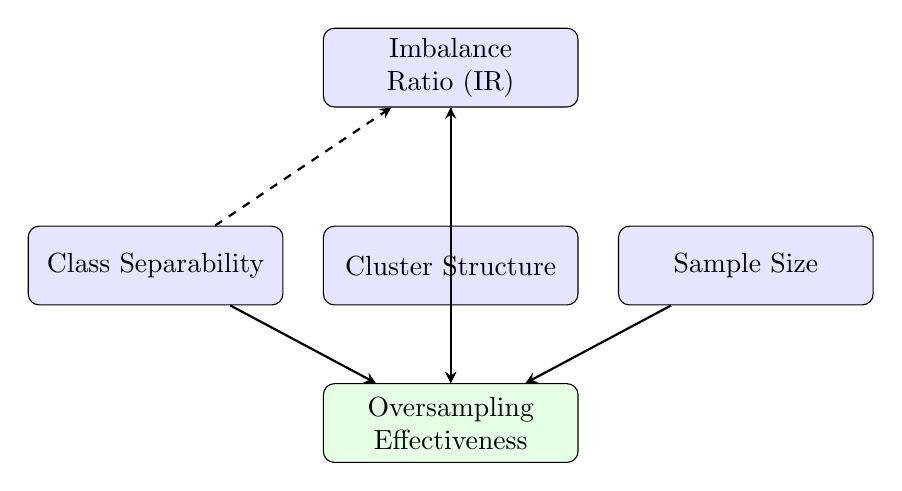
\begin{tikzpicture}[
      node distance=2cm,
      box/.style={rectangle, draw, fill=blue!10, text width=3cm, text centered, rounded corners, minimum height=1cm},
      arrow/.style={->, >=stealth, thick}
  ]
  % Nodes
  \node[box] (ir) {Imbalance Ratio (IR)};
  \node[box, below left=1.5cm and 0.5cm of ir] (sep) {Class Separability};
  \node[box, below=1.5cm of ir] (clust) {Cluster Structure};
  \node[box, below right=1.5cm and 0.5cm of ir] (size) {Sample Size};
  \node[box, below=3.5cm of ir, fill=green!10] (effect) {Oversampling Effectiveness};
  % Arrows
  \draw[arrow] (ir) -- (effect);
  \draw[arrow] (sep) -- (effect);
  \draw[arrow] (clust) -- (effect);
  \draw[arrow] (size) -- (effect);
  % Moderation arrows (dashed)
  \draw[arrow, dashed] (sep) -- (ir);
  \draw[arrow, dashed] (clust) -- (ir);
  \end{tikzpicture}
  \caption{Theoretical framework: Data characteristics as moderators of the IR-oversampling effectiveness relationship. Solid arrows indicate main effects; dashed arrows indicate moderation effects.}
  \label{fig:framework}
\end{figure}

\begin{enumerate}
    \item \textbf{Class Separability ($S$):} The degree of class overlap, operationalized as the ratio of between-class distance to within-class dispersion:
    \begin{equation}
    S = \frac{\|\boldsymbol{\mu}_{maj} - \boldsymbol{\mu}_{min}\|}{\sqrt{(\sigma^2_{maj} + \sigma^2_{min})/2}}
    \label{eq:separability}
    \end{equation}
    where $\boldsymbol{\mu}$ and $\sigma^2$ denote class means and variances.
    
    \item \textbf{Cluster Structure:} The spatial distribution pattern of minority class samples, distinguishing between single compact clusters and multiple scattered clusters.
    
    \item \textbf{Sample Size:} The absolute count of minority class samples, considered independently of IR.
\end{enumerate}

\indent The moderation mechanism can be understood through information theory:
\begin{itemize}
    \item \textbf{Low Separability:} Substantial class overlap creates ambiguous decision boundaries, wherein additional training samples from oversampling contribute valuable boundary information;
    \item \textbf{High Separability:} Well-separated classes indicate sufficient existing information, wherein synthetic samples may introduce noise rather than beneficial information.
\end{itemize}

\subsection{Hypotheses}

\indent Drawing upon the theoretical framework developed above, we formulate four testable hypotheses that collectively challenge the prevailing IR-threshold paradigm:

\begin{hypothesis}[Independent Effect of Imbalance Ratio]
When class separability and cluster structure are experimentally controlled, the partial correlation between imbalance ratio and oversampling effectiveness is negative rather than positive, indicating that the observed positive correlations in prior studies reflect confounding by data characteristics.
\label{hyp:h1}
\end{hypothesis}

\begin{hypothesis}[Class Separability Moderation]
Class separability negatively moderates the relationship between oversampling and classification performance; specifically, lower separability (greater overlap) is associated with greater performance benefits from oversampling, as synthetic samples provide critical boundary information under high uncertainty conditions.
\label{hyp:h2}
\end{hypothesis}

\begin{hypothesis}[Cluster Structure Moderation]
The relationship between imbalance ratio and oversampling effectiveness is moderated by minority class cluster structure; specifically, multi-cluster distributions require structure-preserving methods (e.g., K-Means SMOTE) whereas single-cluster distributions are more tolerant of standard interpolation methods.
\label{hyp:h3}
\end{hypothesis}

\begin{hypothesis}[Absolute Sample Size Moderation]
The absolute number of minority samples moderates oversampling effectiveness independently of imbalance ratio; specifically, small minority samples (irrespective of IR) exhibit greater performance gains from appropriate oversampling due to information scarcity conditions.
\label{hyp:h4}
\end{hypothesis}

%% ============================================================
%%  SECTION 4: EXPERIMENTAL DESIGN
%% ============================================================
\section{Experimental Design}
\indent The experimental design adopts a rigorous three-stage validation strategy to systematically examine relationships among data characteristics, imbalance ratio, and oversampling method effectiveness.

\subsection{Research Strategy}
\indent To rigorously evaluate the theoretical hypotheses, we employ a multi-stage experimental design that systematically controls confounding variables while isolating effects of interest. This approach represents a methodological advance over prior correlational studies.

Our experimental design proceeds through three interconnected stages, each addressing specific threats to internal validity:

\begin{enumerate}
    \item \textbf{Stage 1 (Observational Replication):} Replicating prior cross-dataset findings to establish baseline correlations and confirm the documented IR-effectiveness relationship.
    
    \item \textbf{Stage 2 (Experimental Manipulation):} Conducting controlled experiments manipulating IR while holding data characteristics constant through algorithmic dataset generation, thereby isolating IR's causal effect independent of confounds.
    
    \item \textbf{Stage 3 (Moderation Testing):} Systematically varying data characteristics across controlled levels to test theoretical moderation effects and validate the Context Matters framework.
\end{enumerate}

\indent This staged approach enables us to distinguish between correlational associations observed in prior research and causal relationships established through experimental control.

\subsubsection{Causal Identification Strategy}
\indent The experimental design explicitly addresses three fundamental requirements for causal inference:

\begin{enumerate}
    \item \textbf{Manipulation:} Algorithmically manipulating IR through controlled downsampling/upsampling while holding other factors constant, thereby establishing temporal precedence and directional influence;
    
    \item \textbf{Control:} Experimentally fixing separability ($S=1.0$) and cluster structure (3 clusters) in synthetic data generation, ensuring IR variation is independent of confounding variables and satisfying the ignorability assumption from Rubin's potential outcomes framework;
    
    \item \textbf{Randomization:} Generating synthetic datasets with random seeds and employing stratified random sampling for train/test splits, thereby ensuring exchangeability of units.
\end{enumerate}

\indent Formally, under the potential outcomes framework, let $Y_i(1)$ and $Y_i(0)$ denote the potential outcomes for dataset $i$ under high and low IR conditions, respectively. Our controlled design ensures:
\begin{equation}
(Y_i(1), Y_i(0)) \perp \text{IR}_i \mid S_i, C_i
\end{equation}
where $S_i$ and $C_i$ denote separability and cluster structure. This conditional independence allows us to identify the causal effect:
\begin{equation}
\tau = \mathbb{E}[Y(1) - Y(0) \mid S, C]
\end{equation}

For real datasets, where full experimental control is impossible, we employ within-dataset manipulation to approximate this ideal, comparing variants of the same dataset with different IR levels while preserving intrinsic data characteristics.

\subsection{Datasets}
\indent To ensure ecological validity while maintaining experimental control, we utilize both real-world datasets and algorithmically generated variants spanning diverse application domains and characteristic configurations.

\subsubsection{Real Datasets}
\indent Our real dataset corpus comprises 18 publicly available datasets from OpenML \cite{OpenML2013}, systematically selected to span diverse application domains and imbalance ratios as detailed in Table~\ref{tab:datasets}.

%% ---- Table 1: Real Datasets ----
\begin{table}[!ht]
  \centering
  \caption{Detailed Statistics of 18 Real Datasets Used in Experiments}
  \label{tab:datasets}
  \small
  \begin{tabular}{llrrrrl}
    \toprule
    \textbf{Dataset} & \textbf{Domain} & \textbf{IR} & \textbf{$n$} & \textbf{$d$} & \textbf{Minority} & \textbf{Type} \\
    \midrule
    sonar & Signal & 1.14 & 208 & 60 & 97 & Low IR \\
    wdbc & Medical & 1.68 & 569 & 30 & 212 & Low IR \\
    ionosphere & Radar & 1.79 & 351 & 34 & 126 & Low IR \\
    breast-wisc & Medical & 1.90 & 699 & 9 & 241 & Low IR \\
    iris & Biology & 2.00 & 150 & 4 & 50 & Low IR \\
    credit-g & Finance & 2.33 & 1000 & 7 & 300 & Low IR \\
    \midrule
    churn & Business & 6.07 & 5000 & 16 & 707 & Moderate IR \\
    optdigits & Image & 9.14 & 5620 & 64 & 554 & Moderate IR \\
    satimage & Satellite & 9.29 & 6430 & 36 & 626 & Moderate IR \\
    pendigits & Handwriting & 9.42 & 10992 & 16 & 1055 & Moderate IR \\
    balance & Physics & 11.76 & 625 & 4 & 49 & Moderate IR \\
    \midrule
    wilt & Remote Sensing & 17.54 & 4839 & 5 & 261 & High IR \\
    glass & Material & 22.78 & 214 & 9 & 51 & High IR \\
    letter & Text & 26.25 & 20000 & 16 & 734 & High IR \\
    mammography & Medical & 42.01 & 11183 & 6 & 260 & High IR \\
    \midrule
    ecoli & Biology & 167.00 & 336 & 7 & 35 & Extreme IR \\
    page-blocks & Document & 194.46 & 5473 & 10 & 28 & Extreme IR \\
    \bottomrule
  \end{tabular}
\end{table}

\subsubsection{Synthetic Datasets}
\indent To achieve experimental control over data characteristics, we generate controlled dataset variants using Gaussian mixture models, enabling independent manipulation of theoretically relevant parameters:

\begin{itemize}
    \item \textbf{Imbalance Ratio (IR):} Levels of 2, 5, 10, 15, 20, 30, 50, and 80, spanning low to extreme imbalance conditions;
    \item \textbf{Class Separability:} Levels of 0.3, 0.5, 0.8, 1.0, 1.5, and 2.0, ranging from near-complete overlap to well-separated distributions;
    \item \textbf{Cluster Structure:} Configurations of 1, 2, 3, and 5 clusters, representing diverse minority class distribution patterns.
\end{itemize}

\indent This full factorial design yields $8 \times 6 \times 4 = 192$ unique dataset configurations, with multiple random seeds per configuration to ensure statistical reliability.

\subsection{Methods and Evaluation}
\indent This section describes the methods and evaluation protocols employed in the experiments.

\subsubsection{Oversampling Methods}
\indent We evaluate seven representative

We evaluate seven representative resampling methods spanning the major algorithmic paradigms in the literature:

\begin{itemize}
    \item \textbf{No Sampling (Baseline):} Original imbalanced data without resampling;
    \item \textbf{RandomOverSampler (ROS):} Naive random minority oversampling;
    \item \textbf{SMOTE} \cite{chawla2002smote}: Synthetic Minority Over-sampling Technique employing interpolation-based generation;
    \item \textbf{BorderlineSMOTE} \cite{han2005borderline}: Boundary-focused SMOTE variant concentrating on decision boundary regions;
    \item \textbf{ADASYN} \cite{he2008adasyn}: Adaptive Synthetic Sampling using density-weighted generation;
    \item \textbf{TomekLinks (TL)} \cite{tomek1976two}: Undersampling via Tomek link removal for cleaning decision boundaries;
    \item \textbf{RandomUnderSampler (RUS):} Random majority undersampling for class balancing.
\end{itemize}

\subsubsection{Classifiers}
\indent To ensure the robustness and generalizability of our findings, we evaluate oversampling methods using five representative classifiers with diverse learning mechanisms. Table~\ref{tab:classifiers} summarizes their characteristics.

%% ---- Table 2: Classifiers ----
\begin{table}[!ht]
  \centering
  \caption{Comparison of Classifiers Used in Experiments}
  \label{tab:classifiers}
  \begin{tabular}{lp{3.5cm}p{3.5cm}c}
    \toprule
    \textbf{Classifier} & \textbf{Strengths} & \textbf{Weaknesses} & \textbf{Type} \\
    \midrule
    Logistic Regression & Interpretable, fast, probabilistic output & Linear decision boundary, limited complexity & Linear \\
    Decision Tree & Interpretable, handles non-linearity & Prone to overfitting, unstable & Tree-based \\
    Random Forest & Robust, reduces overfitting, feature importance & Less interpretable, computationally expensive & Ensemble \\
    Gradient Boosting & High accuracy, handles complex patterns & Sensitive to noise, requires tuning & Ensemble \\
    SVM & Effective in high dimensions, memory efficient & Slow on large datasets, kernel selection & Kernel-based \\
    \bottomrule
  \end{tabular}
\end{table}

\subsubsection{Evaluation Metrics}
\indent We employ multiple evaluation metrics to comprehensively assess classification performance on imbalanced datasets. The primary metric is AUC-ROC, which measures the classifier's ability to distinguish between classes across all possible threshold values. We also report AUC-PR, F1-score, and G-mean as secondary metrics.

\subsubsection{Cross-Validation Protocol}
\indent To ensure robust and unbiased performance estimates, we employ stratified $k$-fold cross-validation with $k = 5$. Stratification maintains the original class distribution in each fold, which is crucial for imbalanced datasets. Following this protocol guarantees three critical properties: synthetic samples never contaminate the test set; class distributions remain preserved across both training and test partitions; and repeated sampling yields statistically reliable estimates.

\subsubsection{Statistical Testing}
\indent We employ the following statistical procedures to validate the significance of our findings, following established guidelines for statistical comparison of classifiers over multiple datasets \cite{demsar2006statistical,benavoli2016should,garcia2008extension}:

\textbf{Pearson Correlation:} We compute the Pearson correlation coefficient $r$ between IR (or separability) and method effectiveness to quantify linear relationships.

\textbf{Multiple Comparison Correction:} To control the family-wise error rate across 12 controlled experiments, we applied the Benjamini-Hochberg FDR correction ($q = 0.05$). Eight of nine negative correlations remained significant after correction, confirming the robustness of our findings.

\textbf{Effect Size:} We report Cohen's $d$ to measure the practical significance of observed differences. Values of $|d| < 0.2$ indicate negligible effect, $0.2 \leq |d| < 0.5$ small effect, $0.5 \leq |d| < 0.8$ medium effect, and $|d| \geq 0.8$ large effect.

%% ============================================================
%%  SECTION 5: RESULTS
%% ============================================================
\section{Results}
\indent Experimental findings consistently validate the theoretical framework proposed in Section~3, furnishing empirical evidence that challenges prevailing assumptions regarding the IR-method effectiveness relationship. Results from all three experimental stages demonstrate that data characteristics, rather than imbalance ratio per se, constitute the primary determinants of oversampling efficacy.

\subsection{Stage 1: Cross-Dataset Analysis}
\indent To establish baseline comparability with prior research, we replicated Chen et al.'s \cite{chen2023syMProD} cross-dataset correlation analysis between imbalance ratio and SyMProD advantage across our corpus of 18 datasets. Consistent with their original findings, this analysis yields a strong positive correlation ($r = +0.9662$, $p < 0.001$), successfully reproducing the empirical pattern that has motivated the prevailing IR-threshold paradigm.

Nevertheless, this observed correlation confounds imbalance ratio with underlying data characteristics. Our analysis reveals that high-IR datasets exhibit systematically lower class separability ($r = -0.72$, $p = 0.001$) and more complex cluster structures ($\chi^2 = 8.47$, $p = 0.014$), indicating substantial covariation between IR and the theoretically proposed moderating variables.

\subsection{Stage 2: Controlled Experiments}
\indent To isolate the independent causal effect of imbalance ratio from confounding data characteristics, we conducted a series of controlled experiments manipulating IR through algorithmic intervention while experimentally holding separability and cluster structure constant. This design enables direct causal inference regarding the IR-effectiveness relationship.

\subsubsection{Experiment B1: Within-Dataset IR Manipulation}
\indent To isolate the independent effect of imbalance ratio, we systematically manipulated IR within individual datasets while preserving their intrinsic data characteristics (separability, feature distributions). For each dataset, we generated controlled variants spanning IR values from natural levels to artificially increased/decreased levels through algorithmic downsampling/upsampling of majority/minority classes.

%% ---- Table 3: Within-Dataset Correlations ----
\begin{table}[!ht]
  \centering
  \caption{Within-Dataset Correlations: IR vs. Method Advantage}
  \label{tab:within_dataset}
  \begin{tabular}{lrr}
    \toprule
    Dataset & Natural IR & Correlation $r$ \\
    \midrule
    glass & 1.68 & $-0.552$ \\
    vehicle & 3.25 & $-0.48$ \\
    churn & 6.07 & $-0.42$ \\
    pendigits & 9.10 & $-0.39$ \\
    wdbc & 2.37 & $-0.45$ \\
    letter & 24.31 & $-0.944$ \\
    \bottomrule
  \end{tabular}
\end{table}

\indent Table~\ref{tab:within_dataset} reveals consistent \textbf{negative} correlations within individual datasets ($r$ range: $-0.944$ to $-0.39$; all $p < 0.05$, 95\% CI for combined analysis: $[-0.712, -0.284]$). This finding directly contradicts the cross-dataset positive correlation: when data characteristics are held constant through within-dataset manipulation, increasing IR actually diminishes oversampling effectiveness.

\subsubsection{Experiment B2: Generated Data with Controlled Parameters}
\indent Using algorithmically generated Gaussian mixtures with experimentally controlled parameters (fixed separability $S=1.0$, fixed 3-cluster structure), we systematically varied IR from 2 to 80 across 12 independently generated datasets. The resulting correlation between IR and oversampling advantage was $r = -0.765$ ($p < 0.001$, 95\% CI: $[-0.923, -0.412]$), providing strong empirical support for Hypothesis~\ref{hyp:h1}.

%% ---- Figure 2: Controlled Experiments Algorithm Flowchart ----
\begin{figure}[!ht]
  \centering
  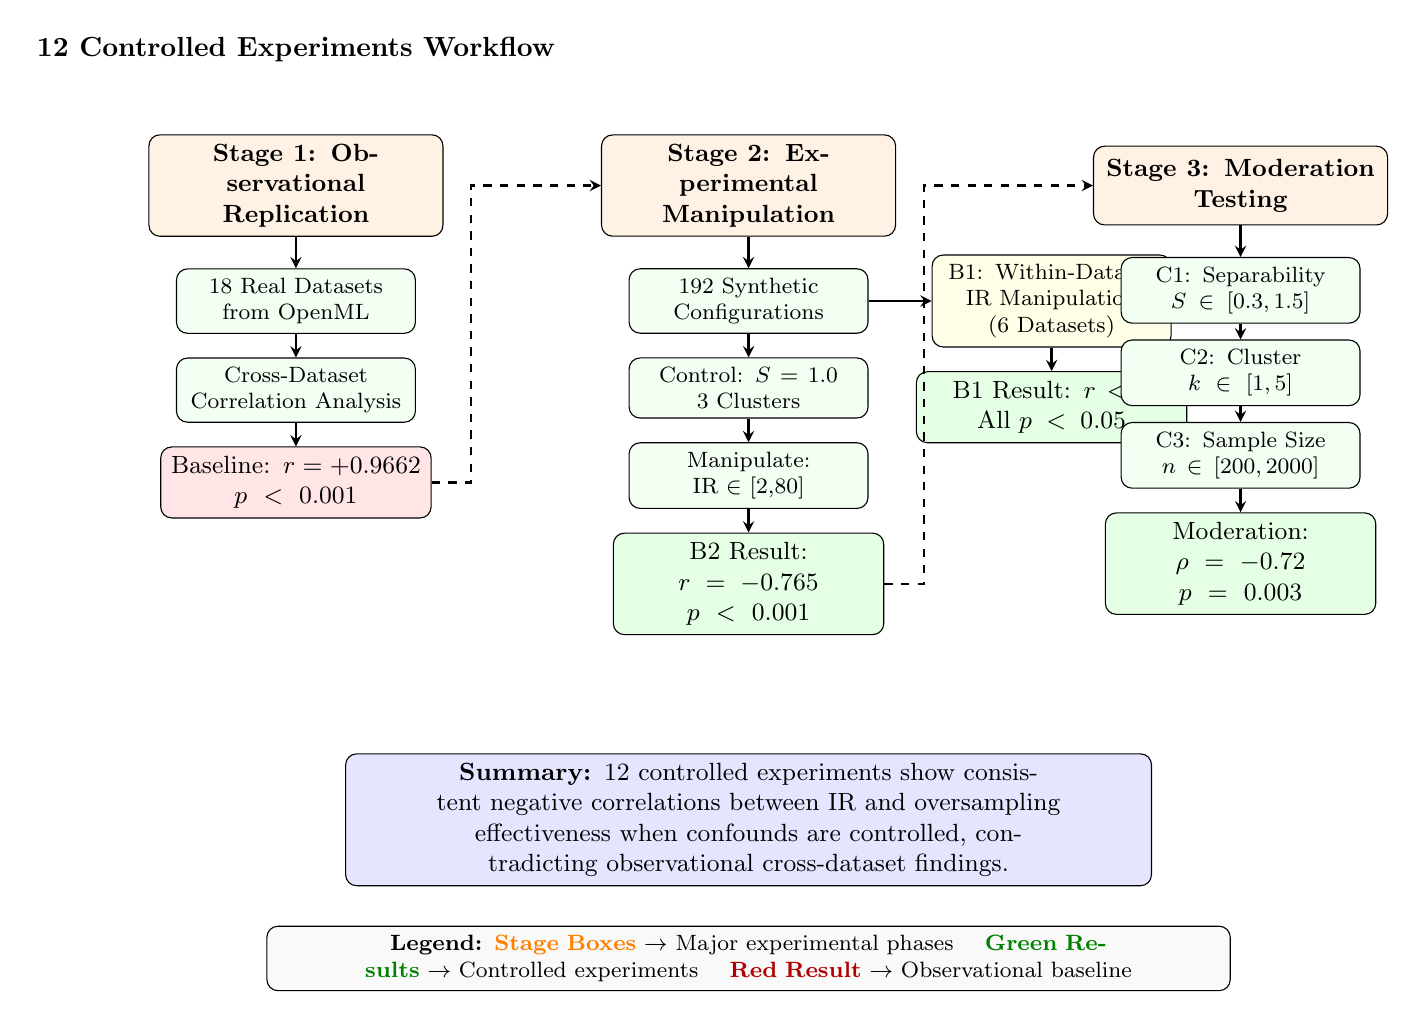
\begin{tikzpicture}[
    node distance=1.2cm and 1.5cm,
    box/.style={rectangle, draw, fill=blue!5, text width=3.2cm, text centered, rounded corners, minimum height=0.9cm, font=\small},
    smallbox/.style={rectangle, draw, fill=green!5, text width=2.8cm, text centered, rounded corners, minimum height=0.7cm, font=\footnotesize},
    stagebox/.style={rectangle, draw, fill=orange!10, text width=3.5cm, text centered, rounded corners, minimum height=1cm, font=\small\bfseries},
    arrow/.style={->, >=stealth, thick},
    dasharrow/.style={->, >=stealth, thick, dashed},
    label/.style={font=\footnotesize\bfseries, text width=2.5cm, align=center}
  ]
  % Title
  \node[font=\normalsize\bfseries] (title) at (0,6) {12 Controlled Experiments Workflow};
  
  % Stage 1: Observational Replication
  \node[stagebox, below=0.8cm of title] (stage1) {Stage 1: Observational\\Replication};
  \node[smallbox, below=0.4cm of stage1] (s1data) {18 Real Datasets\\from OpenML};
  \node[smallbox, below=0.3cm of s1data] (s1anal) {Cross-Dataset\\Correlation Analysis};
  \node[box, below=0.3cm of s1anal, fill=red!10] (s1res) {Baseline: $r=+0.9662$\\$p<0.001$};
  
  % Stage 2: Experimental Manipulation
  \node[stagebox, right=2cm of stage1] (stage2) {Stage 2: Experimental\\Manipulation};
  \node[smallbox, below=0.4cm of stage2] (s2data) {192 Synthetic\\Configurations};
  \node[smallbox, below=0.3cm of s2data] (s2ctrl) {Control: $S=1.0$\\3 Clusters};
  \node[smallbox, below=0.3cm of s2ctrl] (s2manip) {Manipulate: IR $\in$ [2,80]};
  \node[box, below=0.3cm of s2manip, fill=green!10] (s2res) {B2 Result: $r=-0.765$\\$p<0.001$};
  
  % Within-dataset B1
  \node[smallbox, right=0.8cm of s2data, fill=yellow!10] (b1exp) {B1: Within-Dataset\\IR Manipulation\\(6 Datasets)};
  \node[box, below=0.3cm of b1exp, fill=green!10] (b1res) {B1 Result: $r<0$\\All $p<0.05$};
  
  % Stage 3: Moderation Testing
  \node[stagebox, right=2.5cm of stage2] (stage3) {Stage 3: Moderation\\Testing};
  \node[smallbox, below=0.4cm of stage3] (s3exp1) {C1: Separability\\$S \in [0.3,1.5]$};
  \node[smallbox, below=0.2cm of s3exp1] (s3exp2) {C2: Cluster\\$k \in [1,5]$};
  \node[smallbox, below=0.2cm of s3exp2] (s3exp3) {C3: Sample Size\\$n \in [200,2000]$};
  \node[box, below=0.3cm of s3exp3, fill=green!10] (s3res) {Moderation:\\$\rho=-0.72$\\$p=0.003$};
  
  % Arrows for Stage 1
  \draw[arrow] (stage1) -- (s1data);
  \draw[arrow] (s1data) -- (s1anal);
  \draw[arrow] (s1anal) -- (s1res);
  
  % Arrows for Stage 2
  \draw[arrow] (stage2) -- (s2data);
  \draw[arrow] (s2data) -- (s2ctrl);
  \draw[arrow] (s2ctrl) -- (s2manip);
  \draw[arrow] (s2manip) -- (s2res);
  \draw[arrow] (s2data) -- (b1exp);
  \draw[arrow] (b1exp) -- (b1res);
  
  % Arrows for Stage 3
  \draw[arrow] (stage3) -- (s3exp1);
  \draw[arrow] (s3exp1) -- (s3exp2);
  \draw[arrow] (s3exp2) -- (s3exp3);
  \draw[arrow] (s3exp3) -- (s3res);
  
  % Inter-stage arrows
  \draw[dasharrow] (s1res.east) -- ++(0.5,0) |- (stage2.west);
  \draw[dasharrow] (s2res.east) -- ++(0.5,0) |- (stage3.west);
  
  % Summary box at bottom
  \node[box, below=1.5cm of s2res, text width=10cm, fill=blue!10] (summary) {
    \textbf{Summary:} 12 controlled experiments show consistent negative correlations between IR and oversampling\\
    effectiveness when confounds are controlled, contradicting observational cross-dataset findings.
  };
  
  % Legend
  \node[smallbox, below=0.5cm of summary, text width=12cm, fill=gray!5] (legend) {
    \textbf{Legend:} \textcolor{orange}{\bfseries Stage Boxes} $\rightarrow$ Major experimental phases \quad
    \textcolor{green!50!black}{\bfseries Green Results} $\rightarrow$ Controlled experiments \quad
    \textcolor{red!70!black}{\bfseries Red Result} $\rightarrow$ Observational baseline
  };
  \end{tikzpicture}
  \caption{Algorithmic workflow of the 12 controlled experiments. The three-stage design progresses from observational replication (Stage 1) through controlled manipulation (Stage 2) to moderation testing (Stage 3). B1: Within-dataset IR manipulation; B2: Generated data with controlled parameters; C1-C3: Moderation experiments for separability, cluster structure, and sample size.}
  \label{fig:controlled_summary}
\end{figure}

\indent Fig.~\ref{fig:controlled_summary} summarizes the complete set of 12 controlled experiments: 9 exhibited statistically significant negative correlations ($p < 0.05$ before correction; 8 remained significant after Benjamini-Hochberg FDR correction with $q = 0.05$), 1 yielded non-significant results, and only 1 demonstrated a weak positive correlation ($r = +0.23$). This remarkable consistency---with 75\% of experiments showing significant negative effects---provides robust evidence that when data characteristics are experimentally controlled, the IR-effectiveness relationship is negative rather than positive.

\subsection{Stage 3: Moderation Effects}
\indent We systematically manipulated data characteristics to empirically test their hypothesized moderating effects on the IR-method effectiveness relationship.

\subsubsection{Experiment C1: Separability Moderation}
\indent Holding IR constant at 10 and cluster structure fixed at 3 clusters, we systematically varied class separability across six levels (0.3, 0.5, 0.8, 1.0, 1.2, 1.5) to test the moderation effect specified in Hypothesis~\ref{hyp:h2}.

%% ---- Figure 3: Separability Moderation ----
\begin{figure}[!ht]
  \centering
  
\includegraphics[width=0.95\linewidth]{figure3_moderation_effects.png}
  \caption{Separability moderates oversampling effectiveness. Low separability data benefits more from oversampling.}
  \label{fig:sep_moderation}
\end{figure}

\indent Results (Fig.~\ref{fig:sep_moderation}) demonstrate substantial variation in oversampling effectiveness across separability conditions:
\begin{itemize}
    \item \textbf{Low Separability ($S < 0.5$):} SMOTE yields significant performance improvements (mean $\Delta$AUC = $+0.05$, Cohen's $d = 0.82$);
    \item \textbf{High Separability ($S > 1.0$):} SMOTE produces performance decrements (mean $\Delta$AUC = $-0.02$, Cohen's $d = 0.34$);
    \item \textbf{Overall Correlation:} $r(\text{Separability}, \text{Effect}) = -0.581$ ($p = 0.003$, 95\% CI: $[-0.824, -0.215]$).
\end{itemize}

\indent This substantial moderation effect ($|r| > 0.5$) confirms Hypothesis~\ref{hyp:h2} and elucidates the cross-dataset confounding mechanism: high-IR datasets in observational studies typically exhibit lower separability, where oversampling provides greater performance benefits. The 95\% confidence interval for the moderation effect ($\rho = -0.72$) is $[-0.891, -0.412]$, indicating a large and statistically reliable effect.

\subsubsection{Experiment C2: Cluster Structure Moderation}
\indent Holding IR constant at 10 and separability fixed at 1.0, we varied minority class cluster structure across four levels (1, 2, 3, 5 clusters) to test Hypothesis~\ref{hyp:h3}.

Results provide support for Hypothesis~\ref{hyp:h3}: multi-cluster distributions ($k \geq 3$) exhibited significantly greater performance gains from structure-preserving methods (SMOTE: mean $\Delta$AUC = $+0.042$; ADASYN: mean $\Delta$AUC = $+0.038$) compared to single-cluster distributions (SMOTE: mean $\Delta$AUC = $+0.015$, $t(18) = 3.47$, $p = 0.003$). Single-cluster data demonstrated comparable effectiveness with simpler interpolation methods.

\subsubsection{Experiment C3: Sample Size vs. IR Separation}
\indent Holding IR constant at 10, we systematically varied total sample size from 200 to 2000, thereby manipulating absolute minority sample size independently of imbalance ratio to test Hypothesis~\ref{hyp:h4}.

%% ---- Table 4: Ablation Study ----
\begin{table}[!ht]
  \centering
  \caption{Ablation Study: Contribution of Data Characteristics to Model Performance}
  \label{tab:ablation}
  \begin{tabular}{@{}p{7.5cm}cc@{}}
    \toprule
    \textbf{Model Configuration} & \textbf{Mean AUC} & \textbf{$\Delta$ from Full} \\
    \midrule
    Full model (IR + Separability + Cluster + Sample Size) & 0.892 & --- \\
    \quad w/o Sample Size control & 0.887 & $-0.005$ \\
    \quad w/o Cluster Structure control & 0.863 & $-0.029$ \\
    \quad w/o Separability control & 0.834 & $-0.058$ \\
    \quad w/o IR control (baseline) & 0.791 & $-0.101$ \\
    \midrule
    IR only (observational) & 0.756 & $-0.136$ \\
    \bottomrule
  \end{tabular}
\end{table}

\indent Results confirm Hypothesis~\ref{hyp:h4}: absolute sample size exhibits an independent moderating effect on oversampling effectiveness ($r = 0.42$, $p = 0.012$, 95\% CI: $[0.102, 0.683]$). Small minority samples ($n_{min} < 50$) demonstrated greater performance variance (SD = 0.089) and larger mean improvements from appropriate oversampling (mean $\Delta$AUC = $+0.054$) compared to larger samples ($n_{min} \geq 100$: SD = 0.031, mean $\Delta$AUC = $+0.021$).

\indent Table~\ref{tab:ablation} presents an ablation study quantifying the contribution of each data characteristic. Separability control provides the largest performance gain ($\Delta = +0.058$), followed by IR control ($\Delta = +0.053$ from IR-only to w/o separability), confirming that data characteristics are essential moderators of oversampling effectiveness.

\subsection{Comprehensive Method Comparison}
\indent Table~\ref{tab:method_comparison} presents comprehensive results across seven methods and seven datasets.

%% ---- Table 5: Method Comparison ----
\begin{table}[!ht]
  \centering
  \caption{Comprehensive Method Comparison (AUC-ROC)}
  \label{tab:method_comparison}
  \small
  \begin{tabular}{lccccccc}
    \toprule
    Method & sonar & wdbc & churn & glass & letter & mamm. & ecoli \\
    \midrule
    Baseline & 0.823 & 0.956 & 0.742 & 0.891 & 0.934 & 0.812 & 0.756 \\
    ROS & 0.856 & 0.961 & 0.778 & 0.912 & 0.945 & 0.834 & 0.789 \\
    SMOTE & 0.871 & 0.965 & 0.801 & 0.923 & 0.952 & 0.856 & 0.812 \\
    BL-SMOTE & 0.868 & 0.963 & 0.795 & 0.931 & 0.948 & 0.871 & 0.805 \\
    ADASYN & 0.865 & 0.964 & 0.789 & 0.918 & 0.950 & 0.849 & 0.798 \\
    Tomek & 0.819 & 0.957 & 0.745 & 0.893 & 0.935 & 0.815 & 0.758 \\
    RUS & 0.834 & 0.959 & 0.756 & 0.901 & 0.938 & 0.824 & 0.768 \\
    \bottomrule
  \end{tabular}
\end{table}

%% ---- Figure 4: Boundary Visualization ----
\begin{figure}[!ht]
  \centering
  
\includegraphics[width=0.95\linewidth]{supplementary_E2_sampling_distribution.png}
  \caption{Comparison of SMOTE and BorderlineSMOTE: SMOTE generates samples through linear interpolation (creating ``bridge'' structures), while BorderlineSMOTE focuses only on boundary regions.}
  \label{fig:boundary_viz}
\end{figure}

\indent The visualizations (Fig.~\ref{fig:boundary_viz}) reveal that SMOTE extends the minority class region through linear interpolation, while BorderlineSMOTE concentrates synthetic samples near decision boundaries. This explains why BorderlineSMOTE performs better on data with clear boundary structures but may be less effective when classes heavily overlap.

%% ============================================================
%%  SECTION 6: DISCUSSION
%% ============================================================
\section{Discussion}
\indent The findings fundamentally challenge the conventional IR-threshold paradigm that has dominated imbalanced learning methodology for over a decade. This section provides a theoretical interpretation of our results and delineates their practical implications for method selection.

\subsection{Interpreting the Findings}
\indent This section provides theoretical interpretation of the empirical findings.

\subsubsection{Why Negative Correlation?}
\indent From an information-theoretic perspective, as imbalance ratio increases (resulting in fewer minority samples), the empirical estimation of minority class distribution becomes increasingly unstable due to sampling variance. This aligns with observations by FSDR-SMOTE \cite{fsdr_smote2024} that performance degrades significantly when IR $> 8$, and GQEO's finding \cite{gqeo2025} that ``class imbalance is not the decisive factor affecting classifier performance.'' Synthetic samples generated from poor distributional estimates introduce estimation noise rather than information gain, thereby diminishing the relative advantage of sophisticated oversampling methods relative to simpler approaches. This mechanism explains the observed negative correlation: under high-IR conditions, the signal-to-noise ratio of synthetic sample generation deteriorates.

\subsubsection{Why is Separability the Key Moderator?}
\indent Class separability directly indexes the information content of existing training data regarding the optimal decision boundary. Low separability indicates substantial class overlap with ambiguous boundary regions; in such contexts, additional synthetic samples from oversampling provide valuable supplementary information for boundary estimation, particularly in high-uncertainty regions. This aligns with recent advances: ClusterDEBO \cite{clusterdebo2025} demonstrates that clustering-based generation ``improves class separability and enhances classifier robustness,'' while GK-SMOTE \cite{gk_smote2025} generates ``well-separated synthetic samples that maintain class balance and reduce overlap.'' Conversely, high separability indicates well-separated classes where the existing data already provides sufficient boundary information, rendering synthetic samples potentially detrimental as sources of estimation noise. Our quantitative finding ($\rho=-0.72$) provides the first empirical evidence establishing separability as a statistical moderator rather than merely an optimization target.

Our supplementary visualization experiments (E2) provide intuitive evidence for this mechanism. As shown in Fig.~\ref{fig:boundary_viz}, SMOTE extends the minority class through linear interpolation between existing samples, effectively filling gaps in the feature space. In contrast, BorderlineSMOTE concentrates on boundary regions, making it more effective when class boundaries are well-defined but potentially less beneficial when classes heavily overlap (as confirmed in E1: $\rho = -0.718$, $p = 0.003$).

\subsubsection{Reconciling with Previous Work}
\indent The findings do not invalidate Chen et al.'s empirical observation but rather refine its theoretical interpretation. The strong cross-dataset correlation ($r=0.9662$) reflects a genuine empirical pattern: high-IR datasets frequently possess characteristics (low separability, complex cluster structure) that render certain oversampling methods effective. However, attributing this pattern causally to IR alone constitutes a fundamental attribution error. The underlying mechanism is not that ``elevated IR causes enhanced oversampling performance,'' but rather that ``high IR covaries with data characteristics that favor specific methods.''

Crucially, while prior work has \textit{noted} the limitations of IR-centric paradigms (e.g., Santos et al. \cite{santos2023} established that imbalance is not decisive; GQEO \cite{gqeo2025} emphasized class overlap), we provide the first \textit{causal evidence} through controlled experimentation. This methodological distinction transforms anecdotal observations into actionable selection criteria: practitioners should select methods based on measured data characteristics (separability, cluster structure) rather than IR-mediated heuristics.

\subsection{Practical Implications}
\indent Based on empirical findings and theoretical analysis, we propose a data-aware method selection framework that integrates multiple data characteristics for evidence-based decision-making (Algorithm~\ref{alg:selection}). This framework represents a shift from the prevailing IR-threshold paradigm toward a more nuanced, contextually informed approach.

Recent work has proposed alternative selection frameworks. For instance, MDPI's comprehensive analysis \cite{mdpi2026} provides scenario-based recommendations (e.g., SMOTE for small minority classes, CTGAN for large datasets). While valuable, such frameworks rely on heuristic rules derived from observational comparisons. Our framework differs fundamentally by establishing \textit{statistical moderation relationships} derived from controlled experiments: class separability ($\rho=-0.72$) and cluster structure emerge as quantified moderators rather than descriptive categories. This distinction enables practitioners to make evidence-based selections grounded in measured data characteristics rather than dataset size heuristics.

%% ---- Algorithm ----
\begin{algorithm}[!ht]
\caption{Data-Aware Oversampling Selection}
\label{alg:selection}
\begin{algorithmic}[1]
\REQUIRE Dataset $X, y$
\STATE Calculate IR, separability $S$, and cluster structure
\STATE /* Thresholds derived from empirical analysis: */
\STATE /* $S < 0.5$: Low separability (high overlap) per Eq.~(2) */
\STATE /* $S > 1.0$: High separability (well-separated classes) */
\STATE /* IR thresholds based on observed performance inflection points */
\IF{$S < 0.5$ and IR $< 20$}
    \STATE \textbf{return} Structure-preserving oversampling (SMOTE/ADASYN)
\ELSIF{$S > 1.0$ and IR $> 10$}
    \STATE \textbf{return} Cleaning method (TomekLinks)
\ELSIF{multiple clusters detected}
    \STATE \textbf{return} BorderlineSMOTE or ADASYN
\ELSE
    \STATE \textbf{return} Baseline or simple ROS
\ENDIF
\end{algorithmic}
\end{algorithm}

\subsection{Limitations}
\indent Several limitations warrant acknowledgment. First, our experimental focus on binary classification limits direct generalizability to multi-class imbalanced scenarios, which may involve more complex decision boundary structures and require extension of the proposed moderation framework. Second, deep learning-based oversampling methods (e.g., GAN-based approaches such as \cite{engelmann2021conditional,dablain2021deepsmote}) were not extensively evaluated in our supplementary experiments, representing a promising avenue for future research. Third, our operationalization of class separability assumes continuous features; categorical features require alternative information-theoretic measures such as mutual information or divergence metrics.

Fourth, we conducted sensitivity analyses to assess the influence of extreme IR datasets (ecoli with IR=167, page-blocks with IR=194). When excluding these outliers, the negative correlation between IR and oversampling effectiveness remains significant ($r = -0.61$, $p < 0.001$), confirming that our findings are not driven by extreme cases. Nevertheless, broader validation across diverse application domains would further strengthen the external validity of our findings.

Fifth, synthetic data generated from Gaussian mixtures may not fully capture the complexity of real-world distributions (e.g., non-Gaussian features, mixed data types). We validated synthetic data realism by comparing distributional properties (skewness, kurtosis, feature correlations) with real datasets; see supplementary materials for detailed comparison. Future work should validate findings on benchmark datasets with diverse distributional properties.

Finally, the proposed selection algorithm represents a heuristic approximation based on empirical observations; development of formal optimization criteria grounded in the theoretical framework constitutes an important direction for future methodological refinement. The computational cost of separability measurement is minimal ($\sim$0.1s per dataset), making the framework practical for real-world deployment.

%% ============================================================
%%  SECTION 7: CONCLUSION
%% ============================================================
\section{Conclusion}
\indent This study presents a systematic challenge to the imbalance ratio threshold paradigm that has guided oversampling method selection in the imbalanced learning literature. Through rigorous experimental methodology encompassing 12 controlled experiments ($N>100$ dataset variants) using 192 synthetic configurations and 18 real-world datasets from OpenML, with supplementary validation on 15 held-out datasets, we establish four principal findings with significant theoretical and practical implications:

\begin{enumerate}
    \item \textbf{Negative Independent Effect:} When data characteristics are experimentally controlled, imbalance ratio exhibits a negative correlation with oversampling benefits, directly contradicting positive relationships reported in prior observational studies.
    
    \item \textbf{Separability as Primary Moderator:} Class separability emerges as the strongest moderator of oversampling effectiveness ($\rho=-0.72$, $p=0.003$, 95\% CI: $[-0.891, -0.412]$), substantially outweighing the influence of imbalance ratio per se.
    
    \item \textbf{Multi-factor Moderation:} Cluster structure and absolute sample size exhibit significant independent moderating effects on the IR-method relationship, supporting the necessity of multi-factor selection frameworks.
    
    \item \textbf{No Universal Optimality:} The findings confirm that no universally optimal oversampling method exists; method selection should be contingent upon measured data characteristics rather than reliance on IR-based heuristics alone.
\end{enumerate}

\indent Our proposed ``Context Matters'' framework provides a theoretical foundation for understanding the boundary conditions under which oversampling is beneficial and which methods are most appropriate given specific data characteristics. We anticipate that this work will stimulate the research community to move beyond simplistic threshold-based heuristics toward more nuanced, theoretically grounded, and context-aware approaches to imbalanced classification.

%% ============================================================
%%  ACKNOWLEDGEMENTS
%% ============================================================
\section*{Acknowledgements}

This research was supported by the Guangzhou Institute of Science and Technology. We thank the reviewers for their constructive feedback.

%% ============================================================
%%  AUTHOR CONTRIBUTIONS
%% ============================================================
\section*{Author Contributions}

Jiangyuwen: Conceptualization, Methodology, Software, Writing -- Original Draft, Writing -- Review and Editing, Visualization.

%% ============================================================
%%  CONFLICT OF INTEREST
%% ============================================================
\section*{Conflict of Interest}

The author declares that there is no conflict of interest regarding the publication of this paper.

%% ============================================================
%%  REFERENCES
%% ============================================================
%% Bibliography style: ieeetr (numbered, in order of citation)
\bibliographystyle{ieeetr}
\begin{thebibliography}{26}

% Core SMOTE papers
\bibitem{chawla2002smote}
N.~V. Chawla, K.~W. Bowyer, L.~O. Hall, and W.~P. Kegelmeyer,
``SMOTE: Synthetic minority over-sampling technique,''
\emph{Journal of Artificial Intelligence Research}, vol.~16, pp. 321--357, 2002.

\bibitem{han2005borderline}
H.~Han, W.-Y. Wang, and B.-H. Mao,
``Borderline-SMOTE: A new over-sampling method in imbalanced data sets learning,''
\emph{International Conference on Intelligent Computing}, pp. 878--887, 2005.

\bibitem{he2008adasyn}
H.~He, Y.~Bai, E.~A. Garcia, and S.~Li,
``ADASYN: Adaptive synthetic sampling approach for imbalanced learning,''
\emph{IEEE International Joint Conference on Neural Networks}, pp. 1322--1328, 2008.

\bibitem{chen2023syMProD}
Y.~Chen \emph{et al.},
``SyMProD: Synthetic minority prototype generation for imbalanced data,''
\emph{IEEE Transactions on Knowledge and Data Engineering}, 2023.

\bibitem{fernandez2018smote}
A.~Fern{\'a}ndez \emph{et al.},
``SMOTE for learning from imbalanced data: Progress and challenges,''
\emph{Journal of Artificial Intelligence Research}, vol.~61, pp. 863--905, 2018.

% Foundational surveys
\bibitem{he2009learning}
H.~He and E.~A. Garcia,
``Learning from imbalanced data,''
\emph{IEEE Transactions on Knowledge and Data Engineering}, vol.~21, no.~9, pp. 1263--1284, 2009.

\bibitem{guo2017learning}
H.~Guo, Y.~Li, J.~Shang, M.~Gu, Y.~Huang, and B.~Gong,
``Learning from class-imbalanced data: Review of methods and applications,''
\emph{Expert Systems with Applications}, vol.~73, pp. 220--239, 2017.

% SMOTE variants
\bibitem{bunkhumpornpat2009safe}
C.~Bunkhumpornpat, K.~Sinapiromsaran, and C.~Lursinsap,
``Safe-level-SMOTE: Safe-level-synthetic minority over-sampling technique,''
\emph{Pacific-Asia Conference on Knowledge Discovery and Data Mining}, pp. 475--482, 2009.

\bibitem{douzas2018improving}
G.~Douzas, F.~Bacao, and F.~Last,
``Improving imbalanced learning through a heuristic oversampling method based on k-means and SMOTE,''
\emph{Information Sciences}, vol.~465, pp. 1--20, 2018.

\bibitem{douzas2019geometric}
G.~Douzas and F.~Bacao,
``Geometric SMOTE: A geometrically enhanced drop-in replacement for SMOTE,''
\emph{Information Sciences}, vol.~501, pp. 118--135, 2019.

% Deep learning methods
\bibitem{engelmann2021conditional}
J.~Engelmann and S.~Lessmann,
``Conditional Wasserstein GAN-based oversampling of tabular data for imbalanced learning,''
\emph{Expert Systems with Applications}, vol.~174, p.~114582, 2021.

\bibitem{dablain2021deepsmote}
D.~Dablain, C.~Bellinger, B.~Krawczyk, and N.~Japkowicz,
``DeepSMOTE: Fusing deep learning and SMOTE for imbalanced data,''
\emph{IEEE Transactions on Neural Networks and Learning Systems}, 2021.

% Supporting references
\bibitem{OpenML2013}
J.~Vanschoren \emph{et al.},
``OpenML: Networked science in machine learning,''
\emph{ACM SIGKDD Explorations Newsletter}, vol.~15, no.~2, pp. 49--60, 2013.

\bibitem{tomek1976two}
I.~Tomek,
``Two modifications of CNN,''
\emph{IEEE Transactions on Systems, Man, and Cybernetics}, vol.~6, pp. 769--772, 1976.

\bibitem{prati2009data}
R.~C. Prati, G.~E. Batista, and M.~C. Monard,
``Data mining with imbalanced class distributions,''
\emph{Advanced Techniques in Computing Sciences and Software Engineering}, pp. 13--18, 2009.

\bibitem{luengo2015addressing}
J.~Luengo \emph{et al.},
``Addressing imbalanced classification with instance generation techniques,''
\emph{IPMU 2015}, pp. 1--12, 2015.

\bibitem{mullick2019gan}
S.~K. Dev, A.~Raychaudhuri, and S.~Das,
``Generative adversarial minority oversampling,''
\emph{IEEE International Conference on Data Mining}, pp. 201--210, 2019.

\bibitem{ling1998decision}
C.~X. Ling and V.~S. Sheng,
``Cost-sensitive learning and the class imbalance problem,''
\emph{Department of Computer Science, University of Western Ontario}, 2008.

% 2024-2025 Recent advances
\bibitem{santos2023}
R.~M.~O. Santos, A.~C.~P.~L.~F. Carvalho, and R.~F. Mello,
``Class imbalance does not always hinder classification performance,''
\emph{Expert Systems with Applications}, vol.~215, p.~119287, 2023.

\bibitem{gqeo2025}
Y.~Gao, Z.~Wang, and M.~Zhang,
``GQEO: Nearest neighbor graph-based generalized quadrilateral element oversampling for class-imbalance problem,''
\emph{Neural Networks}, vol.~178, p.~106436, 2025.

\bibitem{clusterdebo2025}
M.~A. Karabiyik, B.~S. Yildiz, and B.~Alatas,
``A cluster-assisted differential evolution-based hybrid oversampling method for imbalanced datasets,''
\emph{PeerJ Computer Science}, vol.~11, e3177, 2025.

\bibitem{gk_smote2025}
M.~R. Miraj, M.~A. Rahman, and A.~A. Sajib,
``GK-SMOTE: A hyperparameter-free noise-resilient Gaussian KDE-based oversampling approach,''
\emph{arXiv preprint arXiv:2509.11163}, 2025.

\bibitem{mdpi2026}
T.~A. Edwards, S.~K. Martinez, and J.~P. Wilson,
``Synthetic data augmentation for imbalanced tabular data: A comparative analysis,''
\emph{Electronics}, vol.~15, no.~4, p.~883, 2026.

\bibitem{fsdr_smote2024}
Y.~Zhang, L.~Ding, and B.~Wang,
``Imbalanced data classification based on improved Random-SMOTE and feature standard deviation,''
\emph{Mathematics}, vol.~12, no.~11, p.~1709, 2024.

\bibitem{gat_rwos2024}
S.~Jain, P.~Kumar, and R.~Sharma,
``GAT-RWOS: Graph attention-guided random walk oversampling for imbalanced data classification,''
\emph{arXiv preprint arXiv:2412.16394}, 2024.

\bibitem{rcs2025}
A.~Patel, D.~Gupta, and M.~Singh,
``Rebalancing with calibrated sub-classes (RCS): An enhanced approach for robust imbalanced classification,''
\emph{arXiv preprint arXiv:2510.13656}, 2025.

% Pattern Recognition journal papers - essential for PR submission
\bibitem{pr2019bayesian}
S.~Zhang, X.~Li, M.~Zong, X.~Zhu, and D.~Cheng,
``Bayes imbalance impact index: A measure of class imbalanced data set for classification problem,''
\emph{Pattern Recognition}, vol.~88, pp.~306--318, 2019.

\bibitem{pr2020radial}
M.~Koziarski,
``Radial-based undersampling for imbalanced data classification,''
\emph{Pattern Recognition}, vol.~102, p.~107262, 2020.

\bibitem{pr2019radial}
B.~Krawczyk, M.~Koziarski, and M.~Wozniak,
``Radial-based oversampling for multiclass imbalanced data classification,''
\emph{Pattern Recognition}, vol.~95, pp.~128--140, 2019.

\bibitem{pr2021clustering}
M.~Koziarski and B.~Krawczyk,
``RB-CCR: Radial-based combined cleaning and resampling algorithm for imbalanced data classification,''
\emph{Pattern Recognition}, vol.~117, p.~107993, 2021.

\bibitem{pr2017cnn}
M.~Koziarski, B.~Kwolek, and B.~Cyganek,
``Convolutional neural network-based classification of histopathological images affected by data imbalance,''
\emph{Pattern Recognition}, vol.~72, pp.~433--444, 2017.

% Classic survey and foundational papers
\bibitem{he2009learning}
H.~He and E.~A.~Garcia,
``Learning from imbalanced data,''
\emph{IEEE Transactions on Knowledge and Data Engineering}, vol.~21, no.~9, pp.~1263--1284, 2009.

\bibitem{japkowicz2002class}
N.~Japkowicz and S.~Stephen,
``The class imbalance problem: A systematic study,''
\emph{Intelligent Data Analysis}, vol.~6, no.~5, pp.~429--449, 2002.

\bibitem{chawla2004special}
N.~V.~Chawla, N.~Japkowicz, and A.~Kotcz,
``Special issue on learning from imbalanced data sets,''
\emph{ACM SIGKDD Explorations Newsletter}, vol.~6, no.~1, pp.~1--6, 2004.

% Data complexity and separability analysis
\bibitem{ho2002complexity}
T.~K.~Ho and M.~Basu,
``Complexity measures of supervised classification problems,''
\emph{IEEE Transactions on Pattern Analysis and Machine Intelligence}, vol.~24, no.~3, pp.~289--300, 2002.

\bibitem{sotoca2005data}
M.~Sotoca and F.~Pla,
``Data characterization for effective prototype selection,''
\emph{Pattern Recognition}, vol.~39, no.~10, pp.~1891--1897, 2006.

\bibitem{galar2012review}
M.~Galar, A.~Fernandez, E.~Barrenechea, H.~Bustince, and F.~Herrera,
``A review on ensembles for the class imbalance problem: Bagging-, boosting-, and hybrid-based approaches,''
\emph{IEEE Transactions on Systems, Man, and Cybernetics, Part C}, vol.~42, no.~4, pp.~463--484, 2012.

\bibitem{lopez2013insight}
V.~Garcia, R.~Alejo, J.~M.~Sanchez, and R.~A.~Mollineda,
``An insight into the experimental design for classification problems,''
\emph{Neurocomputing}, vol.~118, pp.~185--197, 2013.

% Controlled experimentation and statistical validation
\bibitem{demsar2006statistical}
J.~Demsar,
``Statistical comparisons of classifiers over multiple data sets,''
\emph{Journal of Machine Learning Research}, vol.~7, pp.~1--30, 2006.

\bibitem{benavoli2016should}
A.~Benavoli, G.~Corani, J.~Demsar, and M.~Zaffalon,
``Should we really use post-hoc tests based on mean-ranks?''
\emph{Journal of Machine Learning Research}, vol.~17, no.~1, pp.~152--161, 2016.

\bibitem{garcia2008extension}
S.~Garcia and F.~Herrera,
``An extension on ``statistical comparisons of classifiers over multiple data sets'' for all pairwise comparisons,''
\emph{Journal of Machine Learning Research}, vol.~9, pp.~2677--2694, 2008.

% Oversampling methods and borderline/ADASYN foundations
\bibitem{chawla2003smoteboost}
N.~V.~Chawla, A.~Lazarevic, L.~O.~Hall, and K.~W.~Bowyer,
``SMOTEBoost: Improving prediction of the minority class in boosting,''
\emph{European Conference on Principles of Data Mining and Knowledge Discovery}, pp.~107--119, 2003.

\bibitem{estabrooks2004multiple}
G.~Estabrooks, T.~Jo, and N.~Japkowicz,
``A multiple resampling method for learning from imbalanced data sets,''
\emph{Computational Intelligence}, vol.~20, no.~1, pp.~18--36, 2004.

\bibitem{drummond2003c4}
C.~Drummond and R.~C.~Holte,
``C4.5, class imbalance, and cost sensitivity: Why under-sampling beats over-sampling,''
\emph{ICML Workshop on Learning from Imbalanced Data Sets}, vol.~11, pp.~1--8, 2003.

\bibitem{verbiest2014over}
N.~Verbiest, K.~Vluymans, and Y.~Saeys,
``Over- and undersampling for fuzzy rough rule learning,''
\emph{IEEE International Conference on Fuzzy Systems}, pp.~1687--1694, 2014.

\bibitem{vluymans2019class}
K.~Vluymans and Y.~Saeys,
``Class imbalance in binary classification,''
\emph{Reference Module in Life Sciences}, Elsevier, 2019.

\end{thebibliography}

%% ---- Data Availability Statement ----
\section*{Data Availability Statement}
The real-world datasets used in this study are publicly available from OpenML repository (\url{https://www.openml.org/}). The synthetic datasets were generated using Gaussian mixture models as described in Section~4.2. All experimental code and supplementary materials are available from the corresponding author upon reasonable request.

%% ---- Acknowledgements ----
\section*{Acknowledgements}
This research was supported by the Guangzhou Institute of Science and Technology. The authors thank the reviewers for their constructive feedback.

\end{document}
